\documentclass[12pt]{article}
\usepackage{amssymb, amsthm, graphics, graphicx}
\usepackage{amsmath}

%these are initial settings. Ron recommended them, so that's just what I use.
\textwidth = 6.5 in
\textheight = 9 in
\oddsidemargin = 0.0 in
\evensidemargin = 0.0 in
\topmargin = -.75in
\parskip = 0.2 in
\parindent = 15 pt
\renewcommand{\baselinestretch}{1.25}

\providecommand{\e}[1]{\ensuremath{\times 10^{#1}}}
\providecommand{\degree}[0]{\ensuremath{^{\circ}}}

\providecommand{\ah}[1]{\ensuremath{\hat{a}_{#1}}}
\providecommand{\ahx}[0]{\ensuremath{\ah{x}}}
\providecommand{\ahy}[0]{\ensuremath{\ah{y}}}
\providecommand{\ahz}[0]{\ensuremath{\ah{z}}}
\providecommand{\pfs}[0]{\ensuremath{\epsilon_{0}}} %permittivity of free space => 1/(36\pi) \e{-9}
%\providecommand{\vec}[1]{\ensuremath{\textbf{#1}}} %vector notation ACTUALLY \vec is _real_ vector notation
\providecommand{\ohm}[0]{\ensuremath{\Omega}}


\newtheorem*{prob}{Problem}

\begin{document}
\begin{flushright}
\textbf{Charles Julian Knight}\\
ECE4893\\
\today
\end{flushright}


\begin{center}
\huge HW 3
\end{center}

\begin{prob}[1.a]{
}\end{prob}
With the 4066 open, the non-inverting input of IC2 is at 
\[\frac{24k}{24k+4.7M}15V \approx .076V\]
Let's call this $V_m$. We've got two inputs into the inverting amp
configuration, so
\[\frac{V_m - V_{saw}}{11k} = \frac{V_{tri}-V_m}{22k} + \frac{-15 - V_m}{82k}\]
\[V_{saw} = -11k \left( \frac{V_{tri}-V_m}{22k} + \frac{-15 - V_m}{82k}\right) + V_m \]
\[ = 1.63V_m - 0.5V_{tri}+2.01V = 2.13V - 0.5V_{tri}\]

\begin{prob}[1.b]{
}\end{prob}
When the 4066 is closed, $V_m$ becomes dependant on $V_{tri}$ also. 
\[V_m = .076 + \frac{56k}{56k+16k}V_{tri} = .076 + .777V_{tri}\]
\[V_{saw} =1.63(.076 + .777V_{tri}) - 0.5V_{tri}+2.01V = 2.14V + .77V_{tri} \]

\begin{prob}[3]{
}\end{prob}
If we apply the ideal opamp rules, what we have is an RC network like this:
\begin{center}
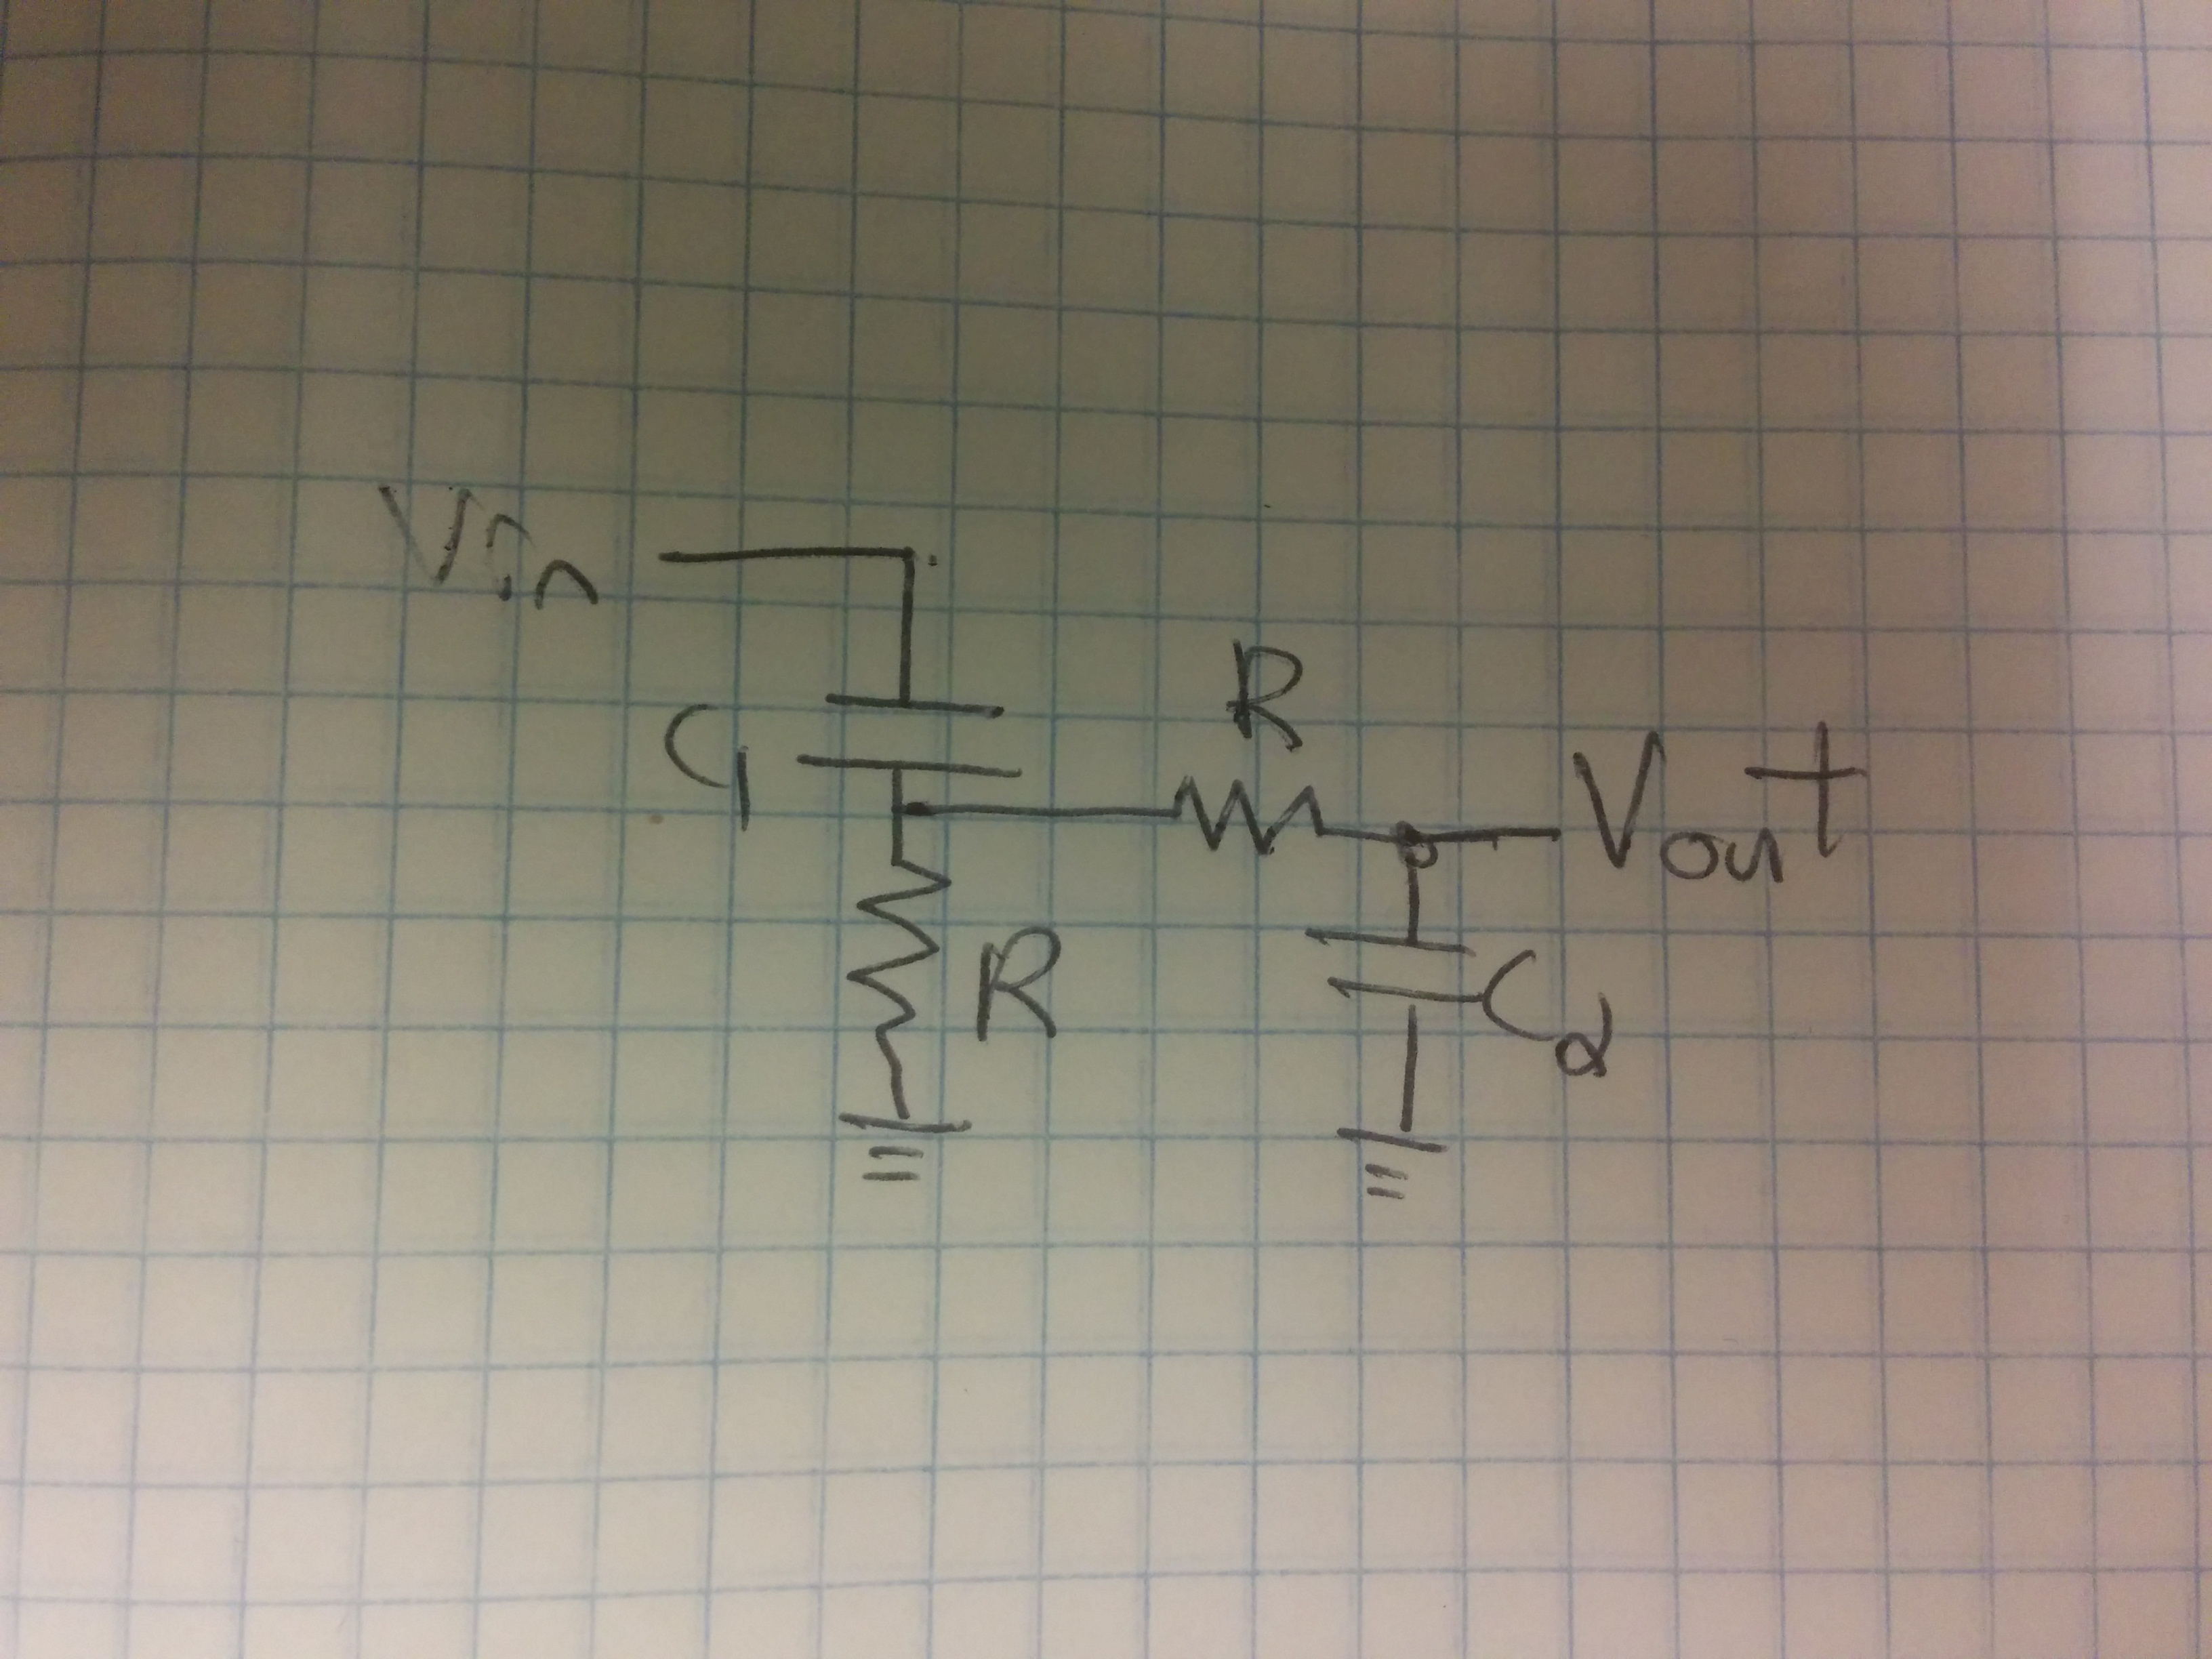
\includegraphics[width=3in]{p3.jpg}
\end{center}
We can look at $V_{out}$ as the cascade of two impedance ladders.
Let's let $Z_1 = 1/sC_1$ and $Z_2=1/sC_2$.
\[V_{out} = \left( \frac{R||(Z_2+R)}{Z_1+R||(Z_2+R)} \right)\left( \frac{Z_2}{R+Z_2} \right)V_{in}\]
%\[V_{out} = \left(\frac{R}{\frac{1}{sC_1}+R}\right)\left(\frac{\frac{1}{sC_2}}{\frac{1}{sC_2}+R}\right)V_{in}\]
%\[T(s) = \frac{V_{out}}{V_{in}} = \frac{ \frac{R}{sC_2} }{ \frac{1}{s^2 C_1 C_2} + \frac{R}{sC_1}+ \frac{R}{sC_2} +R^2 }\]
%Multiplyng top and bottom by $\frac{sC_2}{R}$,
If we dump this into Wolfram$|$Alpha, this simplifies to
\[T(s) = \frac{RZ_2}{R^2 + RZ_2 + 2RZ_1 + Z_1Z_2}\]
If we divide the numerator and denomonator by $RZ_2$,
\[T(s) = \frac{1}{R/Z_2 + 1 + 2Z_1/Z_2 + Z_1/R} = \frac{1}{RC_2s + \frac{1}{RC_1s} + 2C_1/C_2 + 1}\]
\[= \frac{s}{RC_2s^2 + (2C_1/C_2 + 1)s+ \frac{1}{RC_1}}\]
This looks like a bandpass filter as expected. This makes sense, because the signal goes through the capacitor
in the first stage (a high pass pattern).


\end{document}